\documentclass[12pt, a4paper]{article}

% -- Packages -------------------------------------------------
\usepackage[utf8]{inputenc}
\usepackage[T1]{fontenc}
\usepackage{lmodern}
\usepackage{microtype}
\usepackage{geometry}
\geometry{
    a4paper,
    top=2.5cm, bottom=2.5cm,
    left=2.5cm, right=2.5cm
}

\usepackage{amsmath, amssymb}
\usepackage{graphicx}
\usepackage{float}
\usepackage{subcaption}
\usepackage{booktabs}
\usepackage{array}
\usepackage{listings}
\usepackage{xcolor}
\usepackage{tikz}
\usepackage{hyperref}
\usepackage{setspace}
\usepackage{parskip}
\usepackage{titlesec}
\usepackage{fancyhdr}
\usepackage{caption}
\usepackage{enumitem}

% -- Colour palette -------------------------------------------
\definecolor{sectionblue}{RGB}{0, 100, 180}
\definecolor{codebg}{RGB}{248, 248, 248}
\definecolor{codeframe}{RGB}{180, 180, 180}
\definecolor{keywordcolor}{RGB}{0, 0, 200}
\definecolor{commentcolor}{RGB}{60, 140, 60}
\definecolor{stringcolor}{RGB}{160, 0, 0}

% -- Section heading style ------------------------------------
\titleformat{\section}
    {\large\bfseries\color{sectionblue}}
    {\thesection.}{0.5em}{}
    [\vspace{-4pt}\rule{\linewidth}{0.8pt}\vspace{4pt}]

\titleformat{\subsection}
    {\normalsize\bfseries\color{sectionblue}}
    {\thesubsection.}{0.5em}{}

% -- Code listing style ---------------------------------------
\lstset{
    backgroundcolor=\color{codebg},
    basicstyle=\ttfamily\footnotesize,
    keywordstyle=\color{keywordcolor}\bfseries,
    commentstyle=\color{commentcolor}\itshape,
    stringstyle=\color{stringcolor},
    numbers=left,
    numberstyle=\tiny\color{gray},
    stepnumber=1,
    numbersep=6pt,
    frame=single,
    rulecolor=\color{codeframe},
    breaklines=true,
    showstringspaces=false,
    captionpos=b,
    tabsize=4,
}

% -- Hyperref setup -------------------------------------------
\hypersetup{
    colorlinks=true,
    linkcolor=sectionblue,
    urlcolor=sectionblue,
    citecolor=sectionblue,
    pdftitle={Interactive 3D Library Environment Using Modern OpenGL 3.3},
    pdfauthor={[Your Full Name]},
}

% -- Page style ------------------------------------------------
\pagestyle{fancy}
\fancyhf{}
\rhead{\small CSE 4208: Computer Graphics Laboratory}
\lhead{\small 3D Library}
\cfoot{\thepage}
\renewcommand{\headrulewidth}{0.4pt}

% -- Paragraph / spacing --------------------------------------
\setlength{\parindent}{0pt}
\setlength{\parskip}{6pt}

% -- Image placeholder helper ---------------------------------
\newcommand{\imageplaceholder}[2]{
    \fbox{
        \begin{minipage}[c][5.0cm][c]{0.82\textwidth}
            \centering
            \textbf{Image Placeholder}\\[6pt]
            Suggested file: \texttt{#1}\\[6pt]
            \small #2
        \end{minipage}
    }
}

\begin{document}
\pagenumbering{gobble}

\begin{titlepage}
    \centering
    \vspace*{1.5cm}

    {\large\bfseries CSE 4208: Computer Graphics Laboratory}

    \vspace{1.5cm}

    {\Large\bfseries
        Interactive 3D Library Environment \\[6pt]
        Using Modern OpenGL 3.3
    }

    \vspace{3cm}

    {\normalsize Submitted By}\\[8pt]
    {\Large\bfseries [Your Full Name]}\\[4pt]
    {\small Roll: [Your Roll Number]}

    \vspace{3cm}

    % Replace this placeholder with:
    % \includegraphics[width=4cm]{university_logo.png}
    
\begin{tikzpicture}
        \draw[green!60!black, line width=3pt] (0,0) circle (1.8cm);
        \node[align=center, font=\small] at (0,0) {University\\Logo};
    \end{tikzpicture}

    \vfill

    {\normalsize
        Department of Computer Science and Engineering\\[4pt]
        Khulna University of Engineering \& Technology\\[4pt]
        Khulna 9203, Bangladesh
    }
\end{titlepage}

\cleardoublepage
\pagenumbering{arabic}
\setcounter{page}{1}

\section{Abstract}

This project presents an interactive indoor library simulation developed in C++ using Modern OpenGL 3.3. The environment demonstrates the full programmable graphics pipeline through custom GLSL vertex and fragment shaders, indexed mesh rendering, texture mapping, Phong lighting, geometric transformations, and frame-rate-independent animation. The scene is composed primarily from procedurally generated primitive meshes such as cubes, planes, cylinders, spheres, cones, half-tori, and a Bezier surface of revolution used for decorative vases.

The virtual library contains textured walls, floor, ceiling, bookshelves, books, reading tables, chairs, pendant lamps, ceiling fans, a librarian desk, decorative plants, a globe, and a real-time clock. Real-time interaction is provided through first-person camera navigation, mouse look, scroll-based zoom, texture-mode overrides, day-night lighting changes, debug render filters, a bird's-eye orthographic mode, animated fans, and interactive door and window motion. The current version also includes a desk reading lamp with a focused spotlight constrained to the tabletop.

The system is designed for smooth real-time rendering on a standard desktop GPU at 1280$\times$720 resolution, with the exact performance depending on the target machine and driver configuration. The project already demonstrates most core course topics, while future extensions may include shadow mapping, a four-viewport presentation mode, collision-aware interaction, and a custom rotation implementation independent of \texttt{glm::rotate()}.

\section{Introduction}

Real-time 3D graphics programming is a foundational topic in computer graphics because it combines mathematical modelling, linear algebra, lighting theory, data structures, GPU programming, and user interaction into one integrated system. Implementing a complete interactive scene helps reinforce how vertex data moves through the rendering pipeline, how transformations place objects correctly in world space, and how shaders determine the final appearance of surfaces under multiple light sources.

This project models a detailed library reading room with furniture, shelves, lighting fixtures, decorative elements, and animated interactive components. The scene is rendered with OpenGL 3.3 core profile and organized around reusable mesh primitives combined with transformation matrices. Visual realism is improved through texture mapping, material color control, directional daylight, warm pendant point lights, and a desk spotlight that simulates a reading lamp.

The implementation uses GLFW for window creation and input, GLAD for OpenGL function loading, GLM for vector and matrix mathematics, and \texttt{stb\_image} for texture loading. The overall design favors a modular structure: core window/input/shader utilities are separated from renderer primitives and the scene-construction layer, making the project easier to explain, extend, and maintain.

\section{Objectives}

The main objectives of this project are:

\begin{itemize}[leftmargin=1.5em]
    \item Implement a complete Modern OpenGL 3.3 rendering pipeline using shaders, VAOs, VBOs, and EBOs.
    \item Apply translation, rotation, and scaling transformations to construct a complete indoor scene from reusable primitives.
    \item Demonstrate multiple rendering modes including flat color, simple texturing, vertex-stage blending, and fragment-stage blending.
    \item Implement a multi-light Phong illumination system using directional, point, and spotlight sources.
    \item Create a believable library environment with reading tables, chairs, bookshelves, a librarian desk, lamps, decorative objects, and interior architectural elements.
    \item Add real-time animation for ceiling fans, the globe, the wall clock, and interactive door and window motion.
    \item Provide interactive user control through first-person navigation, bird's-eye view, and keyboard-based rendering and lighting toggles.
    \item Demonstrate non-trivial mathematical modelling through a Bezier surface of revolution and an iterative fractal plant generator.
\end{itemize}

\section{System Architecture}

The codebase is organized into a layered architecture with distinct responsibilities. The application entry point initializes the window, OpenGL context, textures, shaders, scene data, and camera. The core layer handles the window, input processing, shader management, and camera math. The renderer layer provides reusable mesh and primitive factories, while the scene layer builds the actual library by instantiating hundreds of lightweight scene objects and a smaller number of unique curved meshes. This separation keeps rendering infrastructure independent from scene-content logic.

Shared state is kept intentionally small. Global runtime state in \texttt{main.cpp} tracks render-mode selection, texture overrides, lighting toggles, fan activity, and bird's-eye mode. The \texttt{Scene} class owns object transforms and animation state, while singleton-style registries are used for shader and texture reuse. The project supports both Visual Studio and CMake-based builds and depends on GLFW, GLAD, GLM, and \texttt{stb\_image}.

\begin{figure}[H]
    \centering
    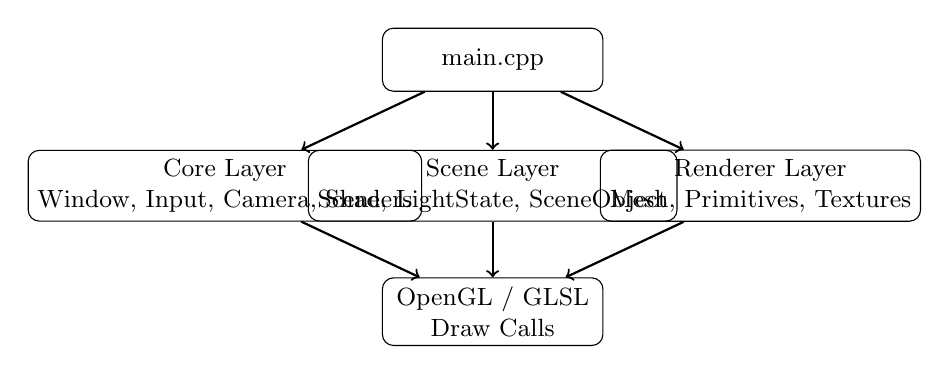
\begin{tikzpicture}[
        box/.style={draw, rounded corners, minimum width=2.8cm,
                    minimum height=0.8cm, align=center, font=\small},
        arr/.style={->, thick}
    ]
        \node[box] (main)   at (0,  3.2) {main.cpp};
        \node[box] (core)   at (-3.4, 1.6) {Core Layer\\Window, Input, Camera, Shaders};
        \node[box] (scene)  at (0,  1.6) {Scene Layer\\Scene, LightState, SceneObject};
        \node[box] (rend)   at (3.4, 1.6) {Renderer Layer\\Mesh, Primitives, Textures};
        \node[box] (gpu)    at (0,  0)   {OpenGL / GLSL\\Draw Calls};
        \draw[arr] (main) -- (core);
        \draw[arr] (main) -- (scene);
        \draw[arr] (main) -- (rend);
        \draw[arr] (core) -- (gpu);
        \draw[arr] (scene) -- (gpu);
        \draw[arr] (rend) -- (gpu);
    \end{tikzpicture}
    \caption{System Architecture Overview}
    \label{fig:architecture}
\end{figure}

\begin{table}[H]
    \centering
    \caption{Main modules and responsibilities}
    \begin{tabular}{lp{9cm}}
        \toprule
        \textbf{File} & \textbf{Role} \\
        \midrule
        \texttt{src/main.cpp} & Program entry point, initialization, render loop, runtime toggles, and per-frame camera/light updates \\
        \texttt{src/core/Window.*} & GLFW window management, OpenGL context setup, event polling, and framebuffer resizing \\
        \texttt{src/core/InputHandler.*} & Keyboard, mouse, and scroll input processing for camera and interaction control \\
        \texttt{src/core/Shader.*} / \texttt{ShaderLibrary.*} & Shader compilation, linking, uniform upload, and registry access for the four shader programs \\
        \texttt{src/renderer/Mesh.*} & VAO/VBO/EBO abstraction for indexed mesh drawing \\
        \texttt{src/renderer/Primitives.*} & Procedural generation of cube, plane, cylinder, sphere, cone, half-torus, and Bezier vase meshes \\
        \texttt{src/renderer/Texture.*} / \texttt{TextureManager.h} & Texture loading, OpenGL texture creation, and reuse by string key \\
        \texttt{src/scene/Scene.*} & Construction, animation, grouping, and rendering of the full library environment \\
        \texttt{src/scene/LightState.h} & Central lighting parameters for directional light, point lights, spotlight, and day-night presets \\
        \bottomrule
    \end{tabular}
    \label{tab:modules}
\end{table}

% =============================================================
%  SECTION 5 -- METHODOLOGY
% =============================================================
\section{Methodology}

\subsection{OpenGL 3.3 Core Rendering Pipeline}

Each frame begins by polling window events and processing continuous user input through the centralized input handler. The application then updates time-dependent animations such as ceiling fan rotation, globe rotation, door opening, window opening, and the real-time wall clock. After that, the current camera state is converted into either a perspective view-projection pair or a bird's-eye orthographic pair, depending on the active viewing mode.

Before rendering, the current light state is uploaded to every shader program used by the scene. The \texttt{Scene} class then traverses two collections: a large array of cube-based \texttt{SceneObject} instances and a smaller array of \texttt{CurvedObject} instances for meshes such as cones, spheres, vases, and the lamp bulb. For each object, the appropriate shader is selected according to its texture mode, the model matrix and material parameters are sent as uniforms, and an indexed draw call is issued through the mesh abstraction.

\begin{figure}[H]
    \centering
    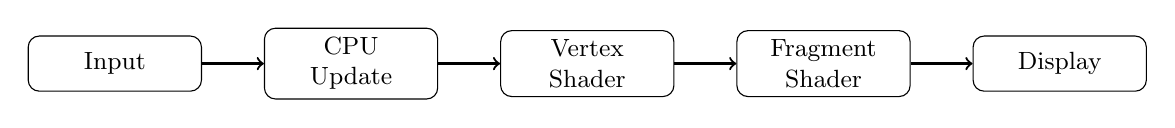
\begin{tikzpicture}[
        stage/.style={draw, rounded corners, minimum width=2.2cm,
                      minimum height=0.7cm, align=center, font=\small},
        arr/.style={->, thick}
    ]
        \node[stage] (in)   at (0,0)    {Input};
        \node[stage] (cpu)  at (3,0)    {CPU\\Update};
        \node[stage] (vs)   at (6,0)    {Vertex\\Shader};
        \node[stage] (fs)   at (9,0)    {Fragment\\Shader};
        \node[stage] (disp) at (12,0)   {Display};
        \draw[arr] (in)--(cpu); \draw[arr] (cpu)--(vs);
        \draw[arr] (vs)--(fs); \draw[arr] (fs)--(disp);
    \end{tikzpicture}
    \caption{Per-frame rendering pipeline}
    \label{fig:pipeline}
\end{figure}

\subsection{Vertex Data and Primitive Geometry}

The entire project uses a single vertex format consisting of position, normal, and UV coordinates. This matches the attribute layout expected by all four shader programs and keeps mesh handling uniform across the project. The cube primitive is the most heavily reused mesh and contains 24 vertices and 36 indices, with separate face vertices so that each face retains a correct normal direction for lighting. The plane primitive contains 4 vertices and 6 indices and is suitable for flat surfaces such as floor or ceiling slabs.

More complex geometry is created procedurally. The cylinder is generated by sweeping a circle along the vertical axis and adding top and bottom caps. The sphere is implemented as a UV sphere using latitude-longitude sampling. The cone is generated as a ruled surface from a base circle to an apex and now supports an optional base cap flag, which is useful for open lampshades. A half-torus is used for the globe stand, and a decorative vase is created by revolving a cubic Bezier profile around the Y-axis. This combination of simple and parametric geometry avoids external model-loading dependencies while still producing a varied scene.

\subsection{Transformation Pipeline}

Every object's transformation follows the standard model--view--projection (MVP) chain:

\begin{equation}
    \mathbf{p}_{\text{clip}} = \mathbf{P} \cdot \mathbf{V} \cdot \mathbf{M} \cdot \mathbf{p}_{\text{model}}
    \label{eq:mvp}
\end{equation}

Here, $\mathbf{M}$ is the object-space model matrix, $\mathbf{V}$ is the camera view matrix, and $\mathbf{P}$ is the projection matrix. In this project, most objects are built from a translation--rotation--scale composition, usually written conceptually as $\mathbf{M} = \mathbf{T}\mathbf{R}\mathbf{S}$. The code stores precomputed model matrices for most static objects, which reduces per-frame CPU work.

Surface normals are transformed using the inverse-transpose of the model matrix:

\begin{equation}
    \mathbf{n}_{\text{world}} = \left(\mathbf{M}^{-1}\right)^{T} \mathbf{n}_{\text{model}}
    \label{eq:normal}
\end{equation}

This is important because many library objects use non-uniform scaling, for example chair legs, shelves, or table supports. Without the inverse-transpose correction, lighting on those objects would appear distorted.

\subsection{Shading Models and Texture Modes}

The project provides four rendering modes that are available both as per-object settings and as a global override. This makes it possible to compare texturing and shading behavior interactively during runtime.

\begin{table}[H]
    \centering
    \caption{Texture and shading modes}
    \begin{tabular}{clp{7cm}}
        \toprule
        \textbf{Mode} & \textbf{Label} & \textbf{Fragment Colour Equation} \\
        \midrule
        0 & Flat color & $\mathbf{c} = \text{Phong}(\mathbf{n}, \mathbf{v}) \times \text{objectColor}$ \\
        1 & Simple texture & $\mathbf{c} = \text{Phong}(\mathbf{n}, \mathbf{v}) \times \text{texColor}$ \\
        2 & Vertex blend & $\mathbf{c} = \text{lighting} \times \bigl((1-\alpha)\,\text{texColor} + \alpha\,\text{objectColor}\bigr)$ with blending prepared at the vertex stage \\
        3 & Fragment blend & $\mathbf{c} = \text{lighting} \times \bigl((1-\alpha)\,\text{texColor} + \alpha\,\text{objectColor}\bigr)$ with blending computed in the fragment stage \\
        \bottomrule
    \end{tabular}
    \label{tab:shading}
\end{table}

These modes are implemented by four GLSL shader pairs: \texttt{basic}, \texttt{texture\_simple}, \texttt{texture\_vertex\_blend}, and \texttt{texture\_fragment\_blend}. Runtime override keys allow the entire scene to be displayed in one mode, which is useful for debugging textures and demonstrating assignment requirements.

\subsection{Lighting Model}

The scene uses a Phong reflection model with three light classes: one directional light to simulate daylight or moonlight, six warm point lights positioned under pendant lamps, and one focused spotlight representing the librarian's reading lamp. All lights share global ambient, diffuse, and specular toggles so the effect of each component can be inspected independently.

The accumulated radiance is:

\begin{equation}
    L = \sum_{i} \frac{1}{k_c + k_l d_i + k_q d_i^2}
        \Bigl( L_{d,i}\max(\hat{n} \cdot \hat{l}_i, 0) + L_{s,i}\max(\hat{r}_i \cdot \hat{v}, 0)^p \Bigr)
    \label{eq:phong}
\end{equation}

In Equation~\ref{eq:phong}, $d_i$ is the distance from the fragment to light $i$, $k_c$, $k_l$, and $k_q$ are the constant, linear, and quadratic attenuation coefficients, $\hat{n}$ is the surface normal, $\hat{l}_i$ is the light direction, $\hat{r}_i$ is the reflected light vector, $\hat{v}$ is the view direction, and $p$ is the shininess exponent. Ambient light is accumulated separately using a global ambient-strength term.

The spotlight deserves special mention. Because the project does not implement shadow mapping, a pure cone-based spotlight would illuminate the floor below the desk as if the desktop were transparent. To solve that limitation, the fragment shaders apply a soft desk-surface mask that constrains the spotlight contribution to the intended reading region on the tabletop.

\subsection{Camera System}

The camera is represented by a world-space position, Euler yaw and pitch angles, a derived front vector, and a field-of-view angle. Mouse motion updates yaw and pitch, keyboard input updates position, and the current view matrix is derived each frame from these values. Scroll input changes the perspective field of view to support zooming.

\begin{itemize}[leftmargin=1.5em]
    \item \textbf{Free first-person camera:} Standard exploration mode with WASD horizontal movement, Q/E vertical movement, mouse look, sprint, and scroll zoom.
    \item \textbf{Bird's-eye orthographic view:} A top-down inspection mode enabled by a dedicated key that replaces the perspective projection with an orthographic projection over the room.
\end{itemize}

\begin{figure}[H]
    \centering
    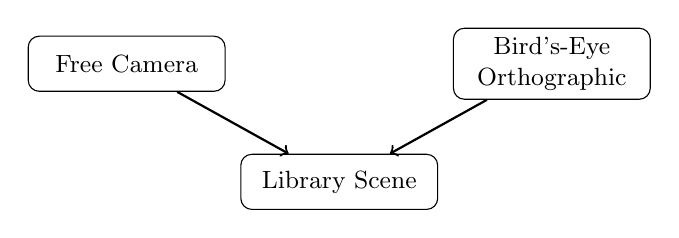
\begin{tikzpicture}[
        box/.style={draw, rounded corners, minimum width=2.5cm,
                    minimum height=0.7cm, align=center, font=\small},
        arr/.style={->, thick}
    ]
        \node[box] (fc) at (-2.7, 1.5) {Free Camera};
        \node[box] (bv) at ( 2.7, 1.5) {Bird's-Eye\\Orthographic};
        \node[box] (sc) at ( 0,   0)   {Library Scene};
        \draw[arr] (fc)--(sc);
        \draw[arr] (bv)--(sc);
    \end{tikzpicture}
    \caption{Implemented camera and view modes}
    \label{fig:camera}
\end{figure}

\subsection{Debug Group Rendering and Global Overrides}

In addition to standard viewing modes, the application supports scene-group isolation and polygon debugging. Function keys can restrict rendering to the room shell, furniture, or shelves and books, while other toggles switch between filled, wireframe, and point-cloud display. This feature is useful during development because it isolates geometry and lighting problems without changing the underlying scene data. Global texture override modes provide a second debugging layer for verifying UV usage and material assignment.

% =============================================================
%  SECTION 6 -- SCENE AND INTERIOR DESIGN
% =============================================================
\section{Scene and Interior Design}

The library is organized as a single enclosed reading room with a strong rectangular plan and a clear interior rhythm. Furniture is distributed in a grid-like arrangement to maintain symmetry and circulation space, while the right-front region is given special emphasis through a librarian desk, a reading lamp, and the wall clock. Decorative objects such as globe stands, vases, and fractal plants break up the repetition of the furniture layout and help the environment feel less mechanical.

\subsection{Library Layout}

The room is approximately 24 units wide, 20 units deep, and 6 units high, based on the current half-width and half-depth scene constants. Reading tables are placed in a 3$\times$3 conceptual grid aligned with the ceiling fan layout, although the front-right table position is intentionally replaced with the librarian desk. Chairs are arranged around the tables, and pendant lamps are suspended above key reading zones. The right wall contains the main door, while side wall openings and windows improve spatial variation and support interaction.

\begin{figure}[H]
    \centering
    % Replace this box with:
    % \includegraphics[width=0.85\textwidth]{images/library_layout_top_view.png}
    \imageplaceholder{images/library_layout_top_view.png}{Capture a bird's-eye or top-view screenshot that clearly shows the full room layout, table grid, librarian desk location, shelves, and door/window placement.}
    \caption{Library layout overview (top or bird's-eye view)}
    \label{fig:layout}
\end{figure}

\subsection{Building Structure}

The structure is an enclosed interior environment consisting of floor, ceiling slab, and surrounding walls with cutouts for windows and the door. Repeated wood and plaster textures are applied to major architectural surfaces, while the door uses a dedicated texture for stronger visual identity. The ceiling hosts both fans and pendant lamps, making it a functional part of the scene rather than a passive boundary plane.

Although the project models a single-room library rather than a multi-storey building, the internal composition still resembles a realistic public reading space. The use of scaled cuboids for walls, frames, shelves, tabletops, and support members provides clean control over dimensions and alignment. This approach also makes the scene easier to modify incrementally.

\subsection{Interior Design}

The interior contains wall-mounted bookshelves filled with repeated book volumes, several reading tables with chairs, ceiling fans, hanging pendant lamps, a dedicated librarian desk, and study materials placed on the desk. The librarian corner includes a more polished desk assembly, executive chair, desk lamp, and a visible desk spotlight. A textured globe and curved decorative objects add variety beyond simple box-based furniture.

\begin{figure}[H]
    \centering
    % Replace this box with:
    % \includegraphics[width=0.75\textwidth]{images/library_interior_view.png}
    \imageplaceholder{images/library_interior_view.png}{Capture an interior perspective showing bookshelves, tables, chairs, pendant lights, and the general reading-room atmosphere.}
    \caption{Interior room view}
    \label{fig:interior}
\end{figure}

\subsection{Additional Features}

Several features enrich the environment beyond basic furniture placement. Two decorative vases use Bezier-generated geometry, and each vase supports an iterative fractal plant composed of many branch and leaf elements. A rotating globe on the librarian desk adds a small motion detail, and the wall clock updates its hands using real system time. Together, these elements improve the realism and help demonstrate both geometric modelling and animation concepts within one cohesive scene.

% =============================================================
%  SECTION 7 -- MATHEMATICAL / ALGORITHMIC FEATURE
% =============================================================
\section{Bezier Surface of Revolution for Decorative Vases}

\subsection{Theory}

The decorative vase is built from a cubic Bezier profile curve revolved about the Y-axis. A cubic Bezier curve is defined by four control points and a parameter $t \in [0,1]$:

\begin{equation}
    \mathbf{B}(t) = (1-t)^3\mathbf{P}_0 + 3(1-t)^2 t\,\mathbf{P}_1
                    + 3(1-t)t^2\,\mathbf{P}_2 + t^3\,\mathbf{P}_3
    \label{eq:feature_main}
\end{equation}

Here, $\mathbf{P}_0$ to $\mathbf{P}_3$ determine the vase silhouette in the radius-height plane. Sampling this curve yields a sequence of profile points, and each point is rotated through $0$ to $2\pi$ around the vertical axis to form a closed surface of revolution.

\begin{equation}
    \mathbf{B}'(t) = 3(1-t)^2(\mathbf{P}_1-\mathbf{P}_0)
    + 6(1-t)t(\mathbf{P}_2-\mathbf{P}_1)
    + 3t^2(\mathbf{P}_3-\mathbf{P}_2)
    \label{eq:feature_secondary}
\end{equation}

The derivative in Equation~\ref{eq:feature_secondary} provides the tangent direction of the profile curve, which is helpful for constructing smooth normals on the generated vase surface.

\subsection{Application to the Scene}

In this project, the Bezier vase is used as a compact decorative container positioned near the library entrance and later paired with fractal plant growth. The Bezier formulation makes it easy to control the base width, body bulge, neck narrowing, and lip opening by editing only four control points. Compared with hard-coded polygon modelling, this method is mathematically cleaner and easier to explain in an academic report.

\begin{lstlisting}[language=C++, caption={Bezier vase generation kernel (adapted from the project primitive factory)}]
glm::vec2 BezierPoint(float t,
                      const glm::vec2& p0,
                      const glm::vec2& p1,
                      const glm::vec2& p2,
                      const glm::vec2& p3) {
    float u = 1.0f - t;
    return u*u*u*p0
         + 3.0f*u*u*t*p1
         + 3.0f*u*t*t*p2
         + t*t*t*p3;
}

void BuildRevolvedProfile(std::vector<Vertex>& vertices,
                          std::vector<unsigned int>& indices,
                          int profileSteps, int radialSlices) {
    for (int i = 0; i <= profileSteps; ++i) {
        float t = static_cast<float>(i) / profileSteps;
        glm::vec2 q = BezierPoint(t, p0, p1, p2, p3);
        for (int j = 0; j <= radialSlices; ++j) {
            float theta = 2.0f * PI * static_cast<float>(j) / radialSlices;
            float x = q.x * std::cos(theta);
            float y = q.y;
            float z = q.x * std::sin(theta);
            // Store position, normal, and UV here
        }
    }
}
\end{lstlisting}

% =============================================================
%  SECTION 8 -- SIMULATION / ANIMATION
% =============================================================
\section{Real-Time Animation and Interaction}

\subsection{Ceiling Fan and Globe Rotation}

The ceiling fans and the desk globe are animated continuously using frame-rate-independent angular updates. Their motion is parameterized by angular velocity, and the current angle is updated each frame based on $\Delta t$, the elapsed time since the previous frame. This guarantees smooth behavior even when the frame rate changes.

\begin{equation}
    \theta_{k+1} = \theta_k + \omega \Delta t
    \label{eq:sim1}
\end{equation}

In Equation~\ref{eq:sim1}, $\theta_k$ is the current rotation angle, $\omega$ is the angular speed in degrees per second, and $\Delta t$ is the frame duration. The same basic update form is used for both the fan blades and the globe, but with different angular velocities so that the globe turns more slowly and feels decorative rather than mechanical.

\begin{figure}[H]
    \centering
    % Replace this box with:
    % \includegraphics[width=0.60\textwidth]{images/fan_or_globe_animation_view.png}
    \imageplaceholder{images/fan_or_globe_animation_view.png}{Capture a screenshot where the rotating fan or globe is clearly visible. A motion-blur-free frame is best for the final report.}
    \caption{Animated fan or globe detail view}
    \label{fig:sim1}
\end{figure}

\subsection{Door and Window Animation}

The door and windows are interactive objects that animate toward open or closed target angles when the user presses the corresponding keys. Instead of teleporting instantly to the new state, the scene updates their transform gradually until the current angle reaches the target. This produces a much more believable interaction and clearly demonstrates state-driven animation.

\begin{equation}
    \theta_{k+1} = \theta_k + \operatorname{sgn}(\theta^\ast - \theta_k)\,
    \min(\omega \Delta t,\lvert \theta^\ast - \theta_k \rvert)
    \label{eq:sim2}
\end{equation}

In Equation~\ref{eq:sim2}, $\theta^\ast$ is the target angle, $\omega$ is the opening speed, and the \texttt{min} term prevents overshoot when the object is close to its destination. This same pattern can be reused for many interactive mechanical elements in real-time graphics applications.

% =============================================================
%  SECTION 9 -- USER CONTROLS
% =============================================================
\section{User Controls}

The project uses keyboard and mouse input through GLFW. Keyboard keys control movement, rendering modes, light states, and interactives, while the mouse controls view direction and the scroll wheel adjusts zoom. The current implementation supports the controls listed in Table~\ref{tab:controls}.

\begin{table}[H]
    \centering
    \caption{Complete keyboard and mouse controls}
    \begin{tabular}{cl}
        \toprule
        \textbf{Key / Input} & \textbf{Function} \\
        \midrule
        W / S & Move camera forward / backward \\
        A / D & Strafe camera left / right \\
        Q / E & Move camera upward / downward \\
        Left Shift & Sprint while moving \\
        Mouse Move & Change camera yaw and pitch \\
        Mouse Scroll & Zoom by changing field of view \\
        Tab & Toggle mouse capture / cursor visibility \\
        F1 & Show all objects \\
        F2 & Render room shell only \\
        F3 & Render furniture only \\
        F4 & Render shelves and books only \\
        F5 & Toggle wireframe mode \\
        F6 & Toggle point-cloud mode \\
        1 & Use per-object texture mode \\
        2 & Force flat-color mode for textured objects \\
        3 & Force simple-texture mode \\
        4 & Force vertex-blend mode \\
        5 & Force fragment-blend mode \\
        T & Cycle texture override mode \\
        L & Toggle all lights on/off \\
        N & Toggle day / night preset \\
        I & Toggle directional light \\
        O & Toggle point lights \\
        6 & Toggle ambient lighting term \\
        7 & Toggle diffuse lighting term \\
        8 & Toggle specular lighting term \\
        G & Toggle ceiling fan animation \\
        B & Toggle bird's-eye orthographic view \\
        H & Toggle door open / close animation \\
        J & Toggle window open / close animation \\
        ESC & Quit application \\
        \bottomrule
    \end{tabular}
    \label{tab:controls}
\end{table}

% =============================================================
%  SECTION 10 -- RESULTS AND OUTPUT
% =============================================================
\section{Results and Output}

\subsection{Visual Quality}

The final scene reproduces a believable indoor library environment with a clear spatial arrangement, consistent material styling, and multiple layers of detail. Key visual outcomes include:

\begin{itemize}[leftmargin=1.5em]
    \item A complete library interior with shelves, books, tables, chairs, pendant lamps, fans, a librarian desk, and decorative objects.
    \item Multiple lighting conditions through directional daylight, night-mode ambience, warm point lights, and a focused desk spotlight.
    \item Procedurally generated curved objects including the globe, open lampshade cone, decorative vases, and lamp bulb geometry.
    \item Interactive and animated elements such as fan motion, globe rotation, door and window opening, and a real-time wall clock.
\end{itemize}

\subsection{Performance}

The application is intended to run interactively at 1280$\times$720 resolution, and the render loop updates the window title with live FPS information during execution. Insert your measured performance here after testing on your final demonstration machine: \textbf{[Measured average FPS at 1280$\times$720 on your target PC]}.

\subsection{Rendered Views}

Different viewpoints should be included in the final report to demonstrate both composition and interaction quality. The placeholders below indicate recommended screenshots to capture.

\begin{figure}[H]
    \centering
    % Replace this box with:
    % \includegraphics[width=0.85\textwidth]{images/birds_eye_view.png}
    \imageplaceholder{images/birds_eye_view.png}{Capture the built-in bird's-eye orthographic view so the overall furniture distribution and symmetry are easy to understand.}
    \caption{Bird's-eye overview of the library}
    \label{fig:splitview}
\end{figure}

\begin{figure}[H]
    \centering
    \begin{subfigure}{0.47\textwidth}
        \centering
        % Replace this box with:
        % \includegraphics[width=\textwidth]{images/front_wall_or_entry_view.png}
        \imageplaceholder{images/front_wall_or_entry_view.png}{Capture a front-facing or entrance-facing scene view.}
        \caption{Entry or front view}
    \end{subfigure}
    \hfill
    \begin{subfigure}{0.47\textwidth}
        \centering
        % Replace this box with:
        % \includegraphics[width=\textwidth]{images/librarian_desk_close_view.png}
        \imageplaceholder{images/librarian_desk_close_view.png}{Capture a close-up of the librarian desk, desk lamp, books, and spotlight.}
        \caption{Desk close-up}
    \end{subfigure}
    \caption{Suggested additional rendered views}
    \label{fig:views}
\end{figure}

% =============================================================
%  SECTION 11 -- CHALLENGES AND SOLUTIONS
% =============================================================
\section{Challenges and Solutions}

\begin{description}[leftmargin=0pt]
    \item[\textbf{Challenge 1 -- Managing a large scene from simple primitives:}]
        Constructing a visually interesting library from mostly cubes and a few procedural meshes can easily lead to repetitive or misaligned geometry. \\
        \textit{Solution:} The scene was organized into dedicated builder functions such as room, shelves, tables, chairs, pendant lamps, librarian desk, and curved objects. Reusable transform helpers and clear object labels kept placement manageable.

    \item[\textbf{Challenge 2 -- Correct lighting under non-uniform scaling:}]
        Many objects use thin scaled cuboids, which can distort lighting if normals are transformed incorrectly. \\
        \textit{Solution:} Normals are transformed using the inverse-transpose of the model matrix in the vertex shader, preserving correct lighting even for highly stretched geometry.

    \item[\textbf{Challenge 3 -- Spotlight leaking under the desk:}]
        The desk lamp spotlight originally illuminated fragments below the tabletop because no geometric shadow system was present. \\
        \textit{Solution:} A desk-surface mask was added in the fragment shaders so the spotlight is constrained to the intended reading patch instead of appearing on the floor.

    \item[\textbf{Challenge 4 -- Visible and believable desk lamp design:}]
        A closed lampshade and misaligned bulb made the reading lamp look visually inconsistent. \\
        \textit{Solution:} The lamp geometry was refined, the cone was opened by making the base cap optional, the bulb was centered on the cone axis, and the spotlight origin was synchronized with the bulb position.
\end{description}

% =============================================================
%  SECTION 12 -- CONCLUSION
% =============================================================
\section{Conclusion}

This project successfully builds an interactive 3D library environment using C++, Modern OpenGL 3.3, GLFW, GLAD, GLM, and GLSL shaders. Through this implementation, the project demonstrates core graphics concepts including indexed mesh rendering, model--view--projection transformations, texture mapping, Phong lighting, camera control, procedural geometry, and interactive animation.

The development process strengthened practical understanding of how separate graphics concepts work together inside a complete real-time application. In particular, the project reinforced the relationship between scene modelling, transformation hierarchies, shader logic, light transport approximations, and user interaction. It also highlighted the importance of code organization when a scene grows to hundreds of objects.

Future improvements may include shadow mapping for more realistic light blocking, a formal four-viewport presentation mode, collision-aware navigation, additional physically motivated materials, and a custom rotation implementation to replace library-provided rotation helpers in selected subsystems.

\section*{References}
\addcontentsline{toc}{section}{References}

\begin{enumerate}[label={[\arabic*]}, leftmargin=2em]
    \item Joey de Vries. \textit{LearnOpenGL}. \url{https://learnopengl.com/}.
    \item GLFW Documentation. \url{https://www.glfw.org/docs/latest/}.
    \item GLAD OpenGL Loader Generator. \url{https://glad.dav1d.de/}.
    \item GLM Documentation. \url{https://glm.g-truc.net/}.
    \item OpenGL Wiki Reference Pages. \url{https://www.khronos.org/opengl/wiki/}.
    \item Sean Barrett. \texttt{stb\_image} image loader. \url{https://github.com/nothings/stb}.
\end{enumerate}

\appendix

\section{Representative Shader Source Snippets}

\begin{lstlisting}[language=GLSL, caption={Vertex Shader excerpt}]
#version 330 core
layout (location = 0) in vec3 aPos;
layout (location = 1) in vec3 aNormal;
layout (location = 2) in vec2 aTexCoord;

uniform mat4 u_Model;
uniform mat4 u_View;
uniform mat4 u_Projection;

out vec3 v_FragPos;
out vec3 v_Normal;
out vec2 v_TexCoord;

void main() {
    vec4 worldPos = u_Model * vec4(aPos, 1.0);
    v_FragPos = vec3(worldPos);
    v_Normal = mat3(transpose(inverse(u_Model))) * aNormal;
    v_TexCoord = aTexCoord;
    gl_Position = u_Projection * u_View * worldPos;
}
\end{lstlisting}

\begin{lstlisting}[language=GLSL, caption={Fragment Shader spotlight-mask excerpt}]
float DeskLampSurfaceMask() {
    const vec2 deskCenter = vec2(6.45, 5.95);
    const vec2 deskRadius = vec2(1.55, 0.82);
    vec2 local = (v_FragPos.xz - deskCenter) / deskRadius;
    float radial = 1.0 - dot(local, local);
    float topMask = smoothstep(0.88, 0.97, v_FragPos.y);
    return max(radial, 0.0) * topMask;
}

vec3 CalcSpotLight(vec3 norm, vec3 viewDir, vec3 baseColor) {
    vec3 lightDir = normalize(u_SpotLightPos - v_FragPos);
    float theta = dot(lightDir, normalize(-u_SpotLightDir));
    float epsilon = u_SpotCutoff - u_SpotOuterCutoff;
    float intensity = clamp((theta - u_SpotOuterCutoff) / epsilon, 0.0, 1.0)
                    * DeskLampSurfaceMask();
    return intensity * baseColor;
}
\end{lstlisting}

\end{document}
